\lstset{ %
language=Python,                % the language of the code
basicstyle=\footnotesize,       % the size of the fonts that are used for the code
backgroundcolor=\color{white},  % choose the background color. You must add \usepackage{color}
showspaces=false,               % show spaces adding particular underscores
showstringspaces=false,         % underline spaces within strings
showtabs=false,                 % show tabs within strings adding particular underscores
frame=single,                   % adds a frame around the code
tabsize=2,                      % sets default tabsize to 2 spaces
captionpos=b,                   % sets the caption-position to bottom
breaklines=true,                % sets automatic line breaking
breakatwhitespace=false,        % sets if automatic breaks should only happen at whitespace
}


\section{Components}

What follows is a listing of application components.

\subsection{Modifications to Freenect}

Done by Jimi.

\subsection{Stereo Calibrate}

Done by Jimi.

\subsection{Creating a model}
\subsubsection{The algorithm}
In stereo calibrate we found two intrinic matrices and two sets of distortion coefficients, two rotation matrices and two translation matrices. All these matrices can be used to undistort both images, so that an object in the depth image is in the same place as an object in the RGB image. We undistort the images using the InitUndistortRectifyMap function from OpenCV. \\
\\
 For now,  \\
We use these corners to determine the orientation of our field. This is done by clicking on the corners in the image we get from the RGB camera, after we undistort the image. 

To create a model of our 3d object we start by determining the field we are going to use. We do that using an A3 sized field with corners that are colored (in order) green, blue, red and black. Now the depth image and the RGB image are aligned and calibrated we can start. The module "create\_model.py" asks the user to click on the pixels in the RGB image, where the corners of the A3 sized workingfield are (see Figure \ref{fig:clicking}). It is important that this is done in the correct order (information is provided in the image).
\begin{figure}[H]
\centering
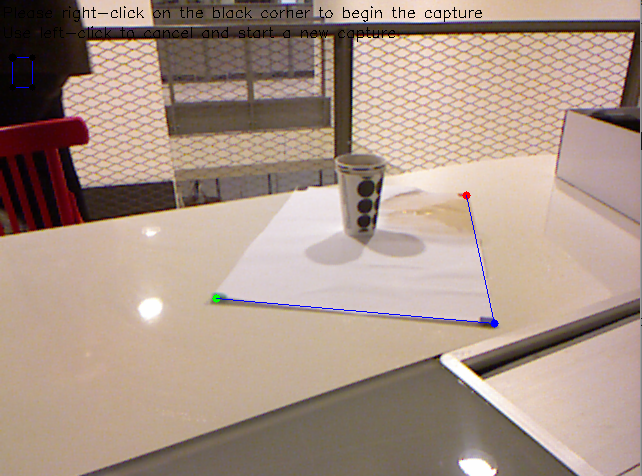
\includegraphics[scale=0.5]{images/clicking.png}
\caption{Clicking on the corners of the working field}
\label{fig:clicking}
\end{figure}
Since we have a depth image, we can make a "working cube" by taking the (x,y,z) value from the points (were the z value is derived from the depth image). The code displayed in \ref{code:cube} is applied to get all 8 points of a cube.\\
\begin{figure}[H]
\begin{lstlisting}
for i in xrange(4):
    cubic.append(np.array([points[i][0],points[i][1],sqrt(depth[points[i][1]][points[i][0]]]), dtype=float))
    if depth[points[i][1]][points[i][0]] > 2000:
        print "Point no. ", i, " is probably in a blind spot. Please start over."


for i in xrange(4):
    cubic = cubic + [np.cross((cubic[((i + 1) % 4)] - cubic[i]),(cubic[((i + 3) % 4)] - cubic[i]))]
    cubic[i + 4] = cubic[i + 4] / np.linalg.norm(cubic[i + 4])
    cubic[i + 4] = (cubic[i + 4] * height) + cubic[i]
\end{lstlisting}
\caption{The algorithm to create a 3 dimensional cube}
\label{code:cube}
\end{figure}
The values of the points we calculate are very rough, so we don't use them later on in our algorithm. We only use the calculated cube to display a wireframe on top of the rgb and depth image, so that the user can determine if the field is correct. At this point, the user can choose to start over or proceed with the points he/she clicked on. \\
\\
All the ingredients to start getting points for our 3d representation in points are now available:\\
\begin{itemize}
\item Four image points (the points we clicked on)
\item A calibrated numpy array containing all RGB values at the moment when the first click was done
\item A calibrated numpy array containing all Depth values at the moment when the first click was done
\end{itemize}
For all points we found in the image, we need to determine the point in the object space. The object space is the cubicle we found earlier, but we didn't determine the axis of the object space. Since we have clicked on all points of the A3 sized plane in a predetermined order, we can choose the axis of our cube. We choose the following: 
\begin{itemize}
\item The origin is in the point above the green corner
\item The x axis is the line that goes threw the origin and the point above the blue corner
\item The y axis is the line that goes threw the origin and the green corner
\item The z axis is the line that goes threw the origin and the point above the black corner
\end{itemize}
The result is visualized in \ref{fig:axis}. 
\begin{figure}[H]
\centering
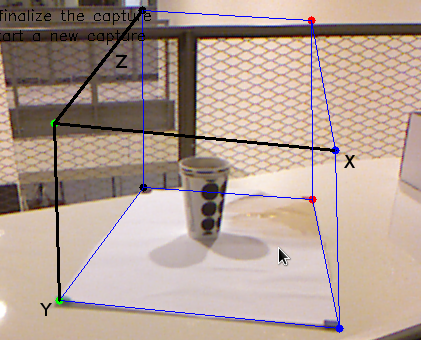
\includegraphics[scale=0.5]{images/axis.png}
\caption{Calculated cube, with axis}
\label{fig:axis}
\end{figure}
We still have to set how large the cube is in object space (in other words, 
how many pixels our 3d object will have). We chose for 100 in the x direction,
100 in the y direction (height of the cube) and 141 for the z direction 
(this is the result of $100 * \sqrt(2)$, which is the ratio of a A3 sized plane).
The points we clicked on can therefore be translated to object space coordinates:\\
$\vec{green} = \left[ \begin{array}{ccc} 
0\\
100\\
0  \end{array} \right] $,
$\vec{blue} = \left[ \begin{array}{ccc} 
100\\
100\\
0  \end{array} \right] $,
$\vec{red} = \left[ \begin{array}{ccc} 
100\\
100\\
141  \end{array} \right] $,
$\vec{black} = \left[ \begin{array}{ccc} 
0\\
100\\
141  \end{array} \right] $\\
The points in object space is the last information we need 
to use the FindExtrinsicCameraParams2 function from opencv. Because we already
undistorted the image in the beginning, we use the identity matrix as the intrinsic 
matrix. For the distortion we can use NULL (same reason). The function returns a
rotation matrix vector and a translation vector. We can make a rotation matrix
from the rotation vector by using the rodrigues2 function in opencv. Together 
with the translation vector, we can make the extrinsic matrix. This is all 
we need for the equation\\
$s \left[ \begin{array}{ccc} 
u\\
v\\
1 \end{array} \right] = 
\left[ \begin{array}{ccc} 
f_{x} & 0 & c_{x}\\
0 & f_{y} & x_{y}\\
0 & 0 & 1 \end{array} \right] 
\left[ \begin{array}{cccc} 
r_{11} & r_{12} & r_{13} & t_{1}\\
r_{21} & r_{22} & r_{23} & t_{2}\\
r_{31} & r_{32} & r_{33} & t_{3} \end{array} \right] 
\left[ \begin{array}{ccc} 
x\\
y\\
z\\
1  \end{array} \right] 
$.\\
In this equation, $\left[ \begin{array}{ccc} 
u\\
v\\
1 \end{array} \right]$ are the image coordinates,\\ $\left[ \begin{array}{ccc} 
x\\
y\\
z\\
1  \end{array} \right] 
$ are the coordinates in object space,\\
$\left[ \begin{array}{ccc} 
f_{x} & 0 & c_{x}\\
0 & f_{y} & x_{y}\\
0 & 0 & 1 \end{array} \right] $ is the intrinsic matrix (identity) and \\
$\left[ \begin{array}{cccc} 
r_{11} & r_{12} & r_{13} & t_{1}\\
r_{21} & r_{22} & r_{23} & t_{2}\\
r_{31} & r_{32} & r_{33} & t_{3} \end{array} \right]$ is the extrinsic matrix.\\\\
Now, because we have to calculate s for every coordinate, we have to do a very
inefficient calculation. We use the above equation for all points in the object
space to determine 
$\left[ \begin{array}{ccc} 
u * s\\
v * s\\
s \end{array} \right] $.\\ We can divide by s, to get the corresponding 
coordinate in the depth image. We go back to the four points we clicked
on. Every point has a corresponding depth value in the depth image. We use
the lowest and the highest value and store them as boundaries. For every 3d
point in the cubicle we check if the corresponding value in the depth image
(first interpolate) is between the boundaries. If so we pass the 3d point to the
point cloud viewer. 
\subsubsection{Defects and TODO}
Defects (at the time of writing):
\begin{itemize}
\item Something goes wrong in the FindExtrinsicCameraParams2, it returns NaN for the translation vector.
\item We still work with distorted images, since the stereo calibration wasn't done.
\item We don't know if the cubicle size is correct.
\item We haven't implemented anything after we needed after FindExtrinsicCameraParams2 because it doesn't work
\end{itemize}
TODO:
\begin{itemize}
\item Undistort and rectify the images
\item Find a replacement for FindExtrinsicCameraParams2
\item Apply the extrinsic matrix to all object points and check if values of those points are between the depth boundaries.
\item Send points to the point cloud viewer
\item Color the points using the rgb image
\item Auto detect the corners of our "working field"
\end{itemize}
\subsection{Point Cloud Viewer}

The point cloud viewer was developed after examining various possible
bases, such as: PCL(see pointclouds.org, A very large production-class project for
anything to do with point clouds), PyGame and Visual. Visual is also know
as VPython.

For a very short period of time we tried using the mpl\_toolkit provided
by matplotlib, but as it has no support for OpenGL it isn't very suited
for rendering a large amount of points in 3D.

The PCL library was of course
very tempting, but very soon it became apparent this was way too much horse
power for our needs. What we needed was a simple interface that allowed viewing
of point clouds, rotating, moving and zooming them with mouse and keyboard
controls.

PyGame allows for very easy initialisation of OpenGL using SDL and can therefore
easily handle point clouds using most of today's graphics hardware. But it still
did not provide an easy way of controlling the camera. Rotation would require
using some sort of mathematical library implementing quaternion spherical rotation.

Enter VPython, a package attempting to implement a simple 3D programming
language on top of Python and allowing interactive terminal control of the
3D scene. VPython officially is composed of: Python (of course), IDLE the
interactive Python programming environment and the visual module. When we
discoverd the visual module used OpenGL, offers mouse orientation
controls by default, and to top it off uses NumPy for all its data manipulation
our course of action became very clear. Since the Kinect library provides its
data in NumPy arrays, after simple manipulation the point clouds can be fed into
visual with the simple command "points".

Currently the point cloud viewer does not support realtime capture, but capture
is done quickly and easily using the 'c' key.


The low-level interface includes the option for depth smoothing.

\subsection{Combining it all}
We have made a Kinect.py module that gives the user a menu. It also takes
arguments. Using arguments, a user can load matrices for undistoring and
rectifying the images from files. If this hasn't been done, the user has to
choose to calibrate first. A user is given the choice by a menu. The second
choice in the menu is to start making a 3d model. This will open the point 
cloud viewer, a rgb screen displaying the image from the rgb camera and a 
depth screen displaying the depth camera. Everytime a user makes a capture,
all points are send to the point cloud viewer. The esc button closes all windows
and brings the user back to the menu.

